\documentclass[xcolor=dvipsnames,hyperref={pdfpagelabels=false}]{beamer}

\usetheme{AnnArbor}

\let\Tiny=\tiny

\newcommand{\bi}{\begin{itemize}}
\newcommand{\ei}{\end{itemize}}
\newcommand{\be}{\begin{enumerate}}
\newcommand{\ee}{\end{enumerate}}
\newcommand{\bc}{\begin{center}}
\newcommand{\ec}{\end{center}}
\newcommand{\I}{\item}
\newcommand{\f}{\frame}
\newcommand{\ft}{\frametitle}
\newcommand{\newIcon}{
\includegraphics[width=0.2in]{new.jpg}}
\newcommand{\checkIcon}{
\includegraphics[width=0.15in]{check_mark.png}}

\title{Hall D Data Flow and Data Challenges}
\subtitle{12 GeV Software Review, 2013}
\author[Mark M.\ Ito]{Mark M.\ Ito}
\date{November 25, 2013}
\institute[JLab]{Jefferson Lab}

\begin{document}

\f{\titlepage}

\section{Outline}

\f{\ft{Outline}
  \bi
  \I Data Flow, Computing Model
    \bi
    \I Raw data taking
    \I Reconstruction
    \I Analysis
    \I Simulation
    \ei
  \I Data Challenges, Past and Future~\newIcon
    \bi
    \I Offline Data Challenges
    \I Online Data Challenges
    \ei
  \ei
  \newIcon $\Rightarrow$ New since last review (June 2012)
}

\section{Data Flow}

\f{\ft{Raw data taking}
  \bi
  \I Detector to Level 3 Farm
    \bi
    \I Monitoring only at first
    \ei
  \I Farm to raid disk in Counting House
  \I EVIO format
  \I transfer to tape library
  \ei
}

\f{\ft{Simulation}
  \bi
  \I on JLab Farm
  \I on the Grid
  \I geometry in XML (HDDS)
  \I using GEANT 3 based detector simulation
  \I conversion to Geant4 well-underway
    \bi
    \I use same geometry
    \I wrap C-based hit generation code from legacy system
    \I facilitate comparisons during transition
    \I overlaps eliminated in geometry~\newIcon
    \ei
  \I Note: resource specification assumes all processing at JLab
    \bi
    \I Reconstruction and Simulation
    \I Use Open Science Grid (OSG) for unanticipated needs, principally simulation
    \ei
  \ei
}

\f{\ft{Reconstruction}
  \bi
  \I JANA framework
    \bi
    \I factory model: reconstructed objects on demand
    \I multi-threaded, event-level parallelization
      \bi
      \I scaling observed up to 32 cores
      \I marginal memory cost per thread 30\% that of single-threaded job
      \ei
    \I calibration constants in relational database
    \ei
  \I REST formatted output~\newIcon
    \bi
    \I an HDDM: compressed XML
    \I compression from raw data: factor of 10
    \I self-documenting
    \I compact
    \ei
  \ei
}

\f{\ft{Analysis Options}
  \bc
  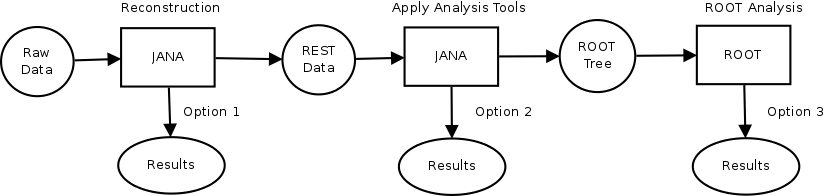
\includegraphics[width=4.5in]{flowchart.png}
  \ec
  \be
  \I During reconstruction in JANA
  \I From REST format in JANA~\newIcon
    \bi
    \I Reconstructed objects re-created on input
    \ei
  \I From ROOT Tree in ROOT~\newIcon
    \bi
    \I Analysis Tools create standard ROOT Trees
    \ei
  \ee
}

\f{\ft{Analysis Tools}
  Library to do standard analysis tasks~\newIcon
    \bi
    \I user specifies reaction of interest (in C++ code) including decays
    \I user does not perform loops and sub-loops over particle combinations
    \I framework returns a list of combinations and their properties
    \I can request kinematic fits of various types
       \bi
       \I energy-momentum conservation
       \I mass constraints
       \I vertex constraints
       \ei
    \I optionally, combinations written to standard ROOT tree
    \I multiple reactions can be specified in same job
    \I already used in studies for PAC 40 proposal
      \bi
      \I demonstrated particle ID using only baseline equipment and kinematics
      \ei
    \ei
}

\section{Data Challenges}

\f{\ft{Data Challenges}
  \newIcon~In cronological order:
  \bi
  \I Data Challenge I: December 2012~\checkIcon
  \I Online Data Challenge I: August 2013~\checkIcon
  \I Data Challenge II: early 2014
  \I Online Data Challenge II: early 2014
  \I Data Challenge III: following DC~II
  \ei
}

  \subsection{Data Challenge I -- December 2012}
    \f{\ft{Data Challenge I: Goals}
      \bi
      \I Produce and handle large data set
        \bi
        \I Generate 2 billion minimum bias events from coherent peak
        \ei
      \I Provide a data sample for kinematics-based particle identification studies (to support PAC 40 proposal)
      \I Look for issues in scaling
      \ei
    }
    \f{\ft{Data Challenge I: Configuration}
      \bi
      \I Minimum-bias hadronic events simulated, only coherent peak
      \I Events simulated and reconstructed in same job
      \I REST format reconstructed written to disk
      \I Raw simulated events discarded
      \I Sites:
        \bc
          \begin{tabular}{l|r}
            \bf Site & \bf Peak \# of Jobs \\
            \hline
            Open Science Grid & 7,000 \\
            JLab Batch Farm & 500 \\
            Carnegie Mellon Cluster & 128
          \end{tabular}
        \ec
      \I At JLab: home-grown workflow tools tailored for JLab environment
        \bi
        \I Other tools seemed too heavy-weight and/or development would be needed
        \I Decision made to defer issue
        \ei
      \ei
    }
    \f{\ft{Data Challenge I: Results}
      \bi
      \I Event count: 5.4 billion events
        \bi
        \I Open Science Grid (OSG): 4.0 billion
        \I Jefferson Lab Batch Farm: 1.0 billion
        \I Carnegie Mellon Nuclear Physics Cluster: 0.4 billion
        \ei
      \I By event count: 2 weeks of data
      \I By usable data: 3 months of data
        \bi
        \I only generated coherent peak $\Rightarrow$ higher ``physics'' purity
        \ei
      \I about 100,000 jobs, about 8 hours each
      \I output REST files: 100 MB/file, 2 kB/event, 10 TB total
      \I Failure rate: about 7\%
        \bi
        \I hangs on single events
        \I segmentation faults
        \I corrupt output data
        \ei
      \ei
    }

    \f{\ft{Grid Usage}
      \bc
      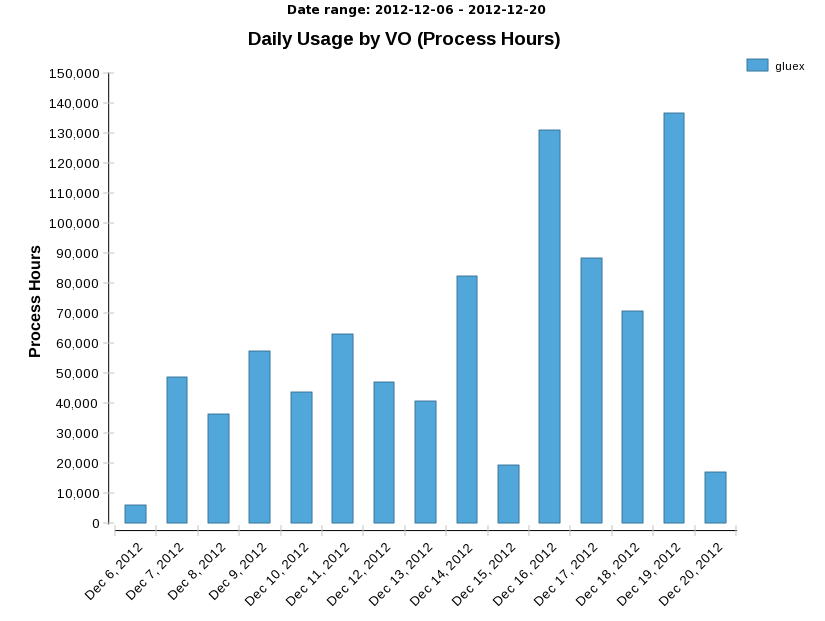
\includegraphics[width=3.5in]{grid_usage_2012.png}
      \ec
    }

    \f{\ft{JLab Farm Usage}
      \bc
      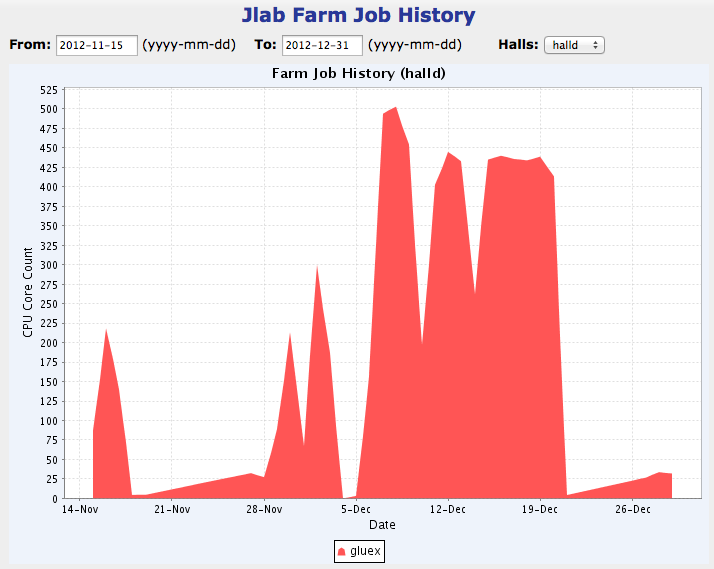
\includegraphics[width=3.5in]{farm_usage_2012.png}
      \ec
    }

    \f{\ft{Example Plot: $\gamma p\rightarrow\pi^+\pi^-\pi^0$}
      \begin{columns}[c]
        \begin{column}{1.2in}
          \small
          \bi
          \I Particle identification cuts applied
          \I With and without cut on kinematic fit confidence level
          \I Cuts and fit performed with Analysis Tools
          \ei
        \end{column}
        \begin{column}{3.3in}
          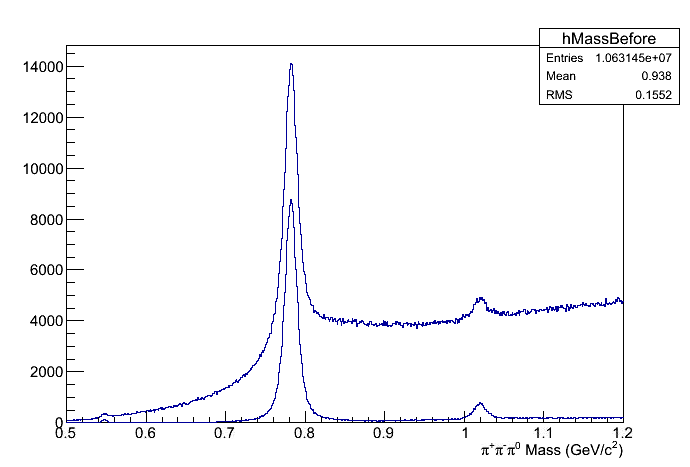
\includegraphics[width=3.3in]{omega_peak.png}
        \end{column}
      \end{columns}
      \bi
      \small
      \I 125 million events from Data Challenge I
      \I 2.4\% of total sample
      \I two days of running at $10^7~\gamma$/s in coherent peak
      \ei
    }
\f{\ft{Data Challenge I: Lessons Learned}
      \bi
      \I Software systems at level that large useful simulated data sets can be produced
        \bi
        \I Data set in fact used: estimated signal vs.\ background (event-level) for several channels of interest involving kaons
        \I Supported main thrust of PAC 40 proposal
        \ei
      \I Need to work hard on bullet-proofing the code
        \bi
        \I failures: contribution to fraction of effort far greater than fraction of failures
        \ei
      \I Tools at JLab need development
        \bi
        \I JLab Scientific Computing Department may help here
        \ei
      \I Need a global (Grid + JLab) meta-data catalog
      \I Need a robust Storage Resource Manager capability at all collaborating institutions
      \ei
    }
  \subsection{Online Data Challenge I -- August 2013}
    \f{\ft{Online Data Challenge I: Goals}
      \bi
      \I Test the RootSpy system in the counting house environment
        \bi
        \I collection of root objects (histograms) from multiple processes
        \ei
      \I Test data rates of EVIO formatted raw data files
      \I Test prototype L3 rejection algorithm
      \I Test data rate to tape library
      \I Monitor health of farm and DAQ system nodes 
      \ei
    }
    \f{\ft{Online Data Challenge I: Configuration}
      \bi
      \I Events pre-staged on disk
      \I Inserted to Event Transfer system (data buffer, supports multiple event producers, multiple event consumers)
      \I Transferred to Level 3 farm, 10~nodes = 80~cores
      \I Nodes mostly borrowed from IT Division
      \I Written to raid disk
      \I Transferred to tape library
      \ei
    }
    \f{\ft{Online Data Challenge I: Results}
      \bi
      \I Level 3 farm measured bandwidth 40 kHz (pass-through)
      \I Simulated HDDM format to EVIO conversion worked; reconstructible events
      \I RootSpy: succeeded
      \ei
    }
    \f{\ft{Level 3 Farm Throughput}
      \begin{columns}[c]
        \begin{column}{1.6in}
          \small
          \bi
          \I Adding ten nodes to the farm, one by one
            \bi
            \I two $\times$ 2.5~GHz Intel Xeon (8~cores, 16~hyperthreads)
            \I eight $\times$ 1.9~GHz AMD Opteron (8~cores)
            \ei
          \ei
        \end{column}
        \begin{column}{2.9in}
          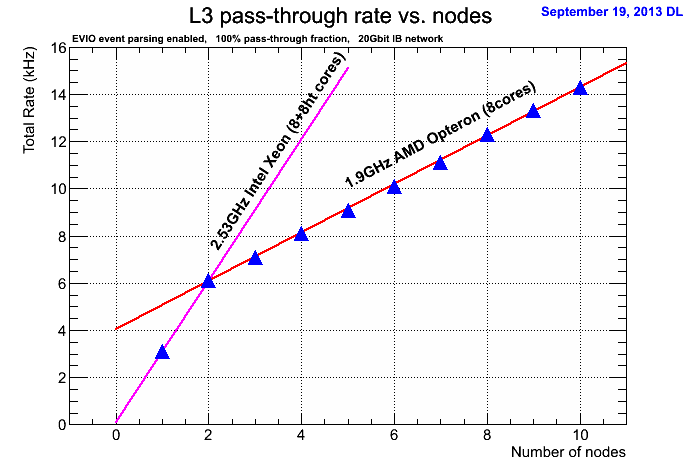
\includegraphics[width=2.9in]{cpu_scaling.png}
        \end{column}
      \end{columns}
      \bi
      \small
      \I Unpacking only: creation of C++ data objects, including translation from geographic to logical addresses
      \I Data ready-to-analyze, but no analysis done
      \I All 10 nodes: 14 kHz, still CPU limited
      \ei
    }
    \f{\ft{Online Data Challenge I: Lessons Learned}
      \bi
      \I Initial Hall D Farm (now installed) can keep up with execution of Level 3 at intensity $10^7\ \gamma$/s
      \I Counting room to tape library transfer should not use standard command-line tool (solved: SciComp method implemented, tested)
      \ei
    }
  \subsection{Future Data Challenges}
    \f{\ft{Data Challenge II -- Early 2014}
      \bi
      \I Goals
        \bi
        \I 10 giga-events
        \I EM background
        \I modern reconstruction
        \I reduce job failure rate
        \ei
      \I Status -- ongoing mini-challenges
      \ei
    }
    \f{\ft{Online Data Challenge II - Early 2014}
      \bi
      \I Goals
        \bi
        \I Test DAQ stream from read-out controllers to tape library
          \bi
          \I stage data in front-end crates
          \ei
        \I Use the full CODA architecture
          \bi
          \I event builder
          \I farm manager
          \I run control
          \ei
        \I Run a realistic Level 3 algorithm in online farm
        \ei
      \I Status -- preparations underway
      \ei
    }
    \f{\ft{Data Challenge III}
      \bi
      \I Two-step process
        \bi
        \I event generation in one set of jobs
        \I reconstruction in independent set of jobs
        \ei
      \I exercises raw data analysis mode
      \I less efficient, may re-use ``raw'' data sets
      \ei
    }
\section{Conclusions}

  \f{\ft{Conclusions}
    \bi
    \I Data Flow plan has remained stable
    \I Addition of REST format since last review
    \I Series of Data Challenges Performed and Planned
      \bi
      \I Done: DC1, ODC1
      \I In preparation: DC2, ODC2, DC3
      \ei
    \I Involvement of IT Division's Scientific Computing Group in collaborative development of workflow/provenance tools
    \I On track to be ready for data taking
    \ei
  }

\section{Backup Slides}

\f{\bc Backup Slides \ec}

\f{
\ft{Data/Computing Model}
Trigger rates:
\bi\scriptsize
\I Phase III: beam rate $10^{7}~\gamma/s$ in coherent peak
\I Full hadronic cross section $\Rightarrow$ 20~kHz trigger rate
\I Beyond Phase III: use level 3 software trigger to keep rate roughly constant
\I Start with ``monitoring farm'', upgrade to ``trigger farm'' 
\ei


Assumptions (generic):
\bi\scriptsize
\I 20 kHz off detector
\I 15 kB events
\I run 35 weeks year, 50\% running efficiency
\I 133 ms to reconstruct an event (measured)
\I 2 Monte Carlo events per data event (on average)
\I 67 ms to generate Monte Carlo events (reconstruction time comparable to data)
\I factor for multiple iterations: 2
\I Other loads:
   \bi\scriptsize
   \I calibration processing
   \I skims/mini-DST production
   \I physics analysis
   \ei
\ei

}

\f{\ft{CPU and Tape Requirements}
\bc
\begin{tabular}{|l|r|r|}
\hline
Process & CPU (kCores) & Tape (PB/y)\\
\hline
Raw Data & -- & 3.2 \\
Calibration & 0.09 & 0.06 \\
Reconstruction & 1.8 & 1.3 \\
Skims/mini-DST & 0.9 & 0.6 \\
Analysis & 0.9 & -- \\
Simulation & 5.4 & 2.5 \\
\hline
Total & 9 & 8 \\
\hline
\end{tabular}
\ec

\small CPU represents amount of computing power required to keep up with average rate off detector. Sets the scale; should be viewed as a minimum requirement.
}
\f{
\ft{Another View of Requirements: Wait Time}

\bc\bf
How long do we wait for results?
\ec

Assume a 10~kCore farm, unloaded, nominal running efficiency, and one iteration only. Other assumptions the same as above.

{\small
\begin{tabular}{lrrr}
 & \bf Phase I & \bf Phase II & \bf Phase III \\
Year of run& 2014 & 2015 & 2016 \\
Days of running & 60 & 60 & 120 \\
Trigger rate (kHz) & 2 & 20 & 20 \\
Number of events & 5.18$\times 10^9$ & 5.18$\times 10^{10}$ & 1.04$\times 10^{11}$ \\
Reconstruction time (days) & 0.8 & 8 & 16 \\
Simulation time (gen.+recon.) (days) & 2.4 & 24 & 48 \\
Recon.+Sim. time (days) & 3.2 & 32 & 64 \\
Total data to tape (PB) & 0.2 &1.8 & 3.6
\end{tabular}
}
}
\frame{
\ft{Open Science Grid (OSG)}

\bi
\I Plan to use Grid resources to augment those at JLab
   \bi
   \I Monte Carlo generation and reconstruction (no raw data transfer)
   \I Opportunistic usage: possible to have quick turn-around on
   specific tasks
   \ei
\I Have established GlueX as a Virtual Organization (VO) with the OSG
\I Nodes from UConn have been contributed
\I Grid Storage Resource Manager (SRM) was used to move data between UConn, Carnegie Mellon, and MIT~\newIcon
\I Effort to grow grid resources coming from university groups
\ei
}

\end{document}

% end of latex file
